\chapter{Case Study}\label{case_study}

The aim of this chapter is to describe the data used to test the models discussed in Chapter\ref{math_model}. The data used in testing is presented in \Cref{data_set}, along with the tools used to obtain it. Furthermore, the different input parameters used in the models are presented in \Cref{key_input_data}. In \Cref{gen_test_inst}, the process of transforming the raw data into usable test instances is discussed. Finally, an example solution to the problem is presented in \Cref{example_solution}.

\section{Data Set}\label{data_set}
To test our model we have used location data from e-scooters in the Oslo area. As there is, to our understanding, no open historic e-scooter location datasets from Oslo, we use the EnTur API to fetch our data. From the ministry of transportation in Norway, EnTur is given the task of making it easier for the Norwegian people to choose a sustainable path with public sector transport (\cite{noauthor_enturno_nodate}). In achieving this goal they have gathered location data from some of the biggest e-scooter companies in Norway, on a standardized form. EnTur provides an API giving a snapshot of all available e-scooters within a specified area. As Oslo is the biggest city in Norway, with the largest number of e-scooters, we have chosen to extract data from this area. Data is fetched from an area with a radius of 20 km from the city center.

To get historical data for demand analysis we have fetched snapshots of available e-scooters every five minutes for a week. This is done to be able to analyze the use patterns of the customers, and henceforth compute the demand and ideal state of different zones. Although demand patterns can vary between weeks, we believe that this data is sufficient to get a sense of customer behavior. Even though it is not performed in this report, further demand analysis could be beneficial to generate improved paths for service vehicles in future research. To create a database with snapshots of locations, we set up a virtual machine at the Google Cloud platform running a script to fetch data and store it in a BigQuery table. The script generated 2016 snapshots from Oslo during a week, consisting of a grand total of 15 720 000 observations of e-scooter positions and battery percentages. This BigQuery table has later been used to run SQL statements to analyze and fetch data for test instances. \Cref{tab:data_example} visualizes the format of the data fetched from the EnTur API.
\\
\begin{table}[h]
    \centering
    \caption{Example of data format in BigQuery}
    \begin{tabular}{|c|c|c|c|c|c|}
        \hline
         \textbf{id} & \textbf{operator} & \textbf{lat} & \textbf{lon} & \textbf{battery} & \textbf{timestamp}  \\
         \hline
         YVO:Scooter:2069... & voi & 59.914928 & 10.747932 & 21.0 & 2020-09-25 09:00:06 \\
         \hline
         YVO:Scooter:293f... & voi & 59.913464 & 10.732058 & 21.0 & 2020-09-25 09:00:06 \\
         \hline
         YTI:Scooter:eab6... & tier & 59.921619 & 10.79154 & 28.0 & 2020-09-25 09:00:06 \\
         \hline
         YTI:Scooter:6aca... & tier & 59.942623 & 10.704265 & 73.0 & 2020-09-25 09:00:06 \\
         \hline
    \end{tabular}
    \label{tab:data_example}
\end{table}

\section{Key Input Data}\label{key_input_data}
The main focus of this report has been the research and development of the mathematical model for the problem described in Chapter \ref{scope and problem description}. The generated input data is used for testing the mathematical model and making sure that everything works. Consequently, the input data is not a completely accurate interpretation of the real world, and following techniques are used to generate input data.

\subsection{Time Distance Matrix}
To calculate the direct distance between locations we have used the latitude and longitude from the EnTur data. For simplification purposes the direct distance is used to test the model, instead of more accurate distances through the city centre. The distance between two coordinates is computed using the haversine formula. Formula \eqref{eq:haversine} shows the expression for the distance between two points. $r$ is the radius of the earth while $\phi_{1}$ , $\phi_{2}$, $\delta_{1}$ and $\delta_{2}$ are the geographical coordinates given as latitude and longitude.

\setcounter{equation}{0}
\begin{equation}\label{eq:haversine}
    d = 2r\arcsin\left(\sqrt{\sin^2\left(\frac{\phi_{2}-\phi_{1}}{2}\right)+ \cos(\phi_{1})\cos(\phi_{2})\sin^2\left(\frac{\delta_{2}-\delta_{1}}{2}\right)}\right)
\end{equation}

After computing the distance, $d$, from Formula \eqref{eq:haversine}, a proxy for the time taken per distance is used to compute the time distance. The average speed within the center of Oslo is around 40 km/h (\cite{fosli_effekter_1999}). However, since the service vehicles will be idle for about half of the operating time, we have reduced this proxy to 20 km/t. This is an approximation and not an accurate proxy, but takes into account both time of travel and time of performing battery swaps, pick-ups, and deliveries, and will suffice for testing purposes.

\subsection{Reward Function}\label{reward function}
The reward function awarding battery swaps and rebalancing moves are calculated based on the battery percentage. For each battery swap, we get a reward equal to one minus the e-scooter battery percentage. Further, the delivery locations receive a reward equal to one if they are visited. This is due to the assumption that all rebalanced e-scooters get a battery swap, as discussed in \Cref{assumptions}. Formula \eqref{eq:standard_reward} sums up the explained schema for the values of the reward, where the reward given is equal to the battery capacity added by visiting each location. The reward can thus also be interpreted as the amount of additional availability the fleet of e-scooters experiences after a visit to a given location. The battery capacity of the e-scooters are obtained from the EnTur dataset.

\begin{equation}\label{eq:standard_reward}
    R_{i} = \begin{cases}
        1-B_{i} & \textbf{if }\text{$i$ is an e-scooter location} \\
        1 & \textbf{if }\text{$i$ is a delivery location} \\
        0 & \textbf{if }\text{$i$ is a depot location}
    \end{cases}
\end{equation}

For the alternative model, a function with diminishing returns for adding more e-scooters to a zone is used. This is introduced to incentivize the model to perform battery swaps and move e-scooters to zones far away from their ideal state. Formula \eqref{eq:alternative_reward} shows the function used to compute the reward. 
\begin{equation}
    \begin{split}\label{eq:alternative_reward}
        R_{kz} = \begin{cases} 
            R_{(k-1)z} + \beta + \theta\left(\frac{D^I_z}{k}\right) & \textbf{if}\quad k \geq 1, D^I_z \geq 0  \text{ and } R_{(k-1)z} \leq 1\\
            1 & \textbf{if} \quad k \geq 1, D^I_z \geq 0  \text{ and } R_{(k-1)z} > 1\\
            0 & otherwise
        \end{cases} \\
    \end{split}
    \\\nonumber
    \\
    \text{ where } D^I_z = I_z - \displaystyle\sum_{i\in \mathcal{L}_z} B_i \nonumber
\end{equation}

$k$ denotes the number of locations that are visited in a given zone, while $I_z$ is the ideal state of that zone. $B_i$ is the battery percentage of the e-scooter in location $i$. Thus, $D^I_z$ represents the deviation from the ideal state in zone $z$. The reward is only given in zones below its ideal state, as the reward is set to 0 for zones where the deviation is negative. $\beta$ denotes the part of the reward for visiting one additional location that is independent of $k$. $\theta$ captures how much the function diminishes as more locations are visited in a zone. A high value of $\theta$ makes the last location visited in a zone yield a lower reward than the first. A low value means that the deviation between the reward given for the first and last location visited is smaller. The reward of the alternative model is visualized in \Cref{fig:alt_reward_function} with the parameters listed in \Cref{tab:param_reward_function}.
\\
\begingroup
    \setlength{\tabcolsep}{10pt} % Default value: 6pt
    \renewcommand{\arraystretch}{1.9} % Default value: 1
    \begin{table}[h]
        \centering
        \caption{Parameters used in reward function in \Cref{fig:alt_reward_function}}
        \begin{tabular}{c|c}
            
             \textbf{Parameter} & \textbf{Numerical Value}   \\
             \hline
             $I_z$ & 10\\
             \hline
             $\sum_{i\in \mathcal{L}_z} B_i$ & 7\\
             \hline
             $\beta$ & 0.4\\
             \hline
             $\theta$ & 0.4 \\
             
        \end{tabular}
        \label{tab:param_reward_function}
    \end{table}
\endgroup

\begin{figure}[H]
    \centering
    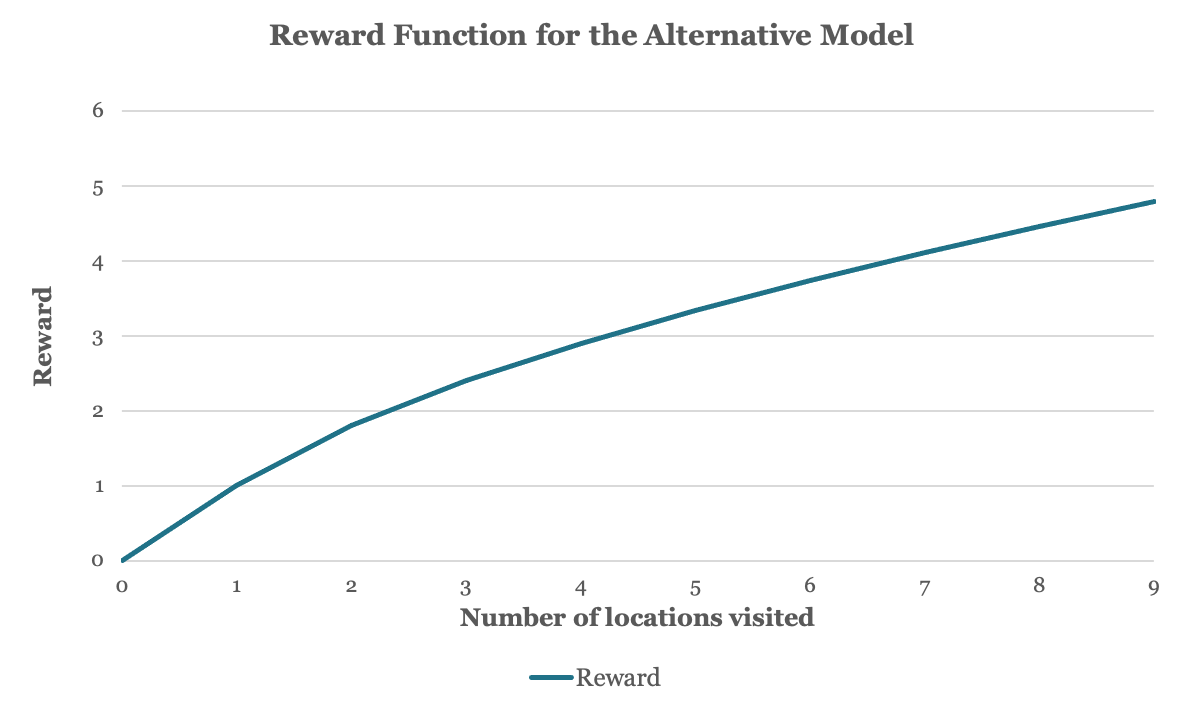
\includegraphics[width=0.8\columnwidth]{Images/alt_reward.png}
    \caption{Visualization of the reward function of the alternative model}
    \label{fig:alt_reward_function}
\end{figure}

For the example instance described in \Cref{tab:param_reward_function}, the marginal reward for each additional location visited quickly converges towards the value of $\beta$. This is  because of the relatively low deviation between the ideal state and the total battery capacity in the zone looked at. Although visiting four location yields a reward of 2.9, visiting one additional location only yield an extra reward of 0.44. Thus, the model would be incentivized to rather travel to a different zone with a larger deviation from the ideal state. For example, visiting five locations in a zone with no battery capacity available and the same ideal state as in \Cref{tab:param_reward_function}, would yield a reward of 5.0. Note that the battery capacity of the e-scooters in the locations visited would be subtracted from the overall reward in the objective function, as shown in \Cref{alt_model}.
    

\section{Generation of Test Instances}\label{gen_test_inst}
For the purpose of testing the model, a series of methods have been used to generate viable test instances. To provide a valid instance the following steps are performed:
\begin{enumerate}
    \item Input size of the test instance
    \item Create zones and e-scooter nodes
    \item Generate delivery nodes
    \item Choose an appropriate shift duration and vehicle capacities
\end{enumerate}
In this subsection, a description of how these steps are performed is provided. All instances use data from a subsection of the Oslo EnTur data from the city center. The data in use is a single snapshot taken at 09:00 at 25-09-2020. The bounds of the coordinate system used are defined by a crop of the city map of Oslo. All e-scooters within these bounds are shown in \Cref{fig:all_data}.
\\
\begin{figure}[h]
    \centering
    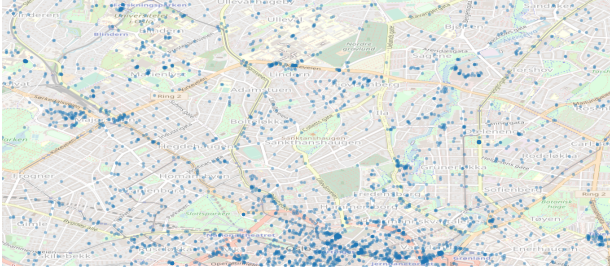
\includegraphics[width=0.8\columnwidth]{Images/all_data.png}
    \caption{Map with all e-scooters within the cropped area.}
    \label{fig:all_data}
\end{figure}

\subsection{Zones and Locations}
A new test instance is generated by specifying  $\textit{Number of Sections}$ and  $\textit{Number of E-scooters per Zone}$. These numbers define the size of an instance. Equations \Cref{eq:sectionsEquations} give a summary of the size of an instance based on the input arguments.
\\
\begin{equation}\label{eq:sectionsEquations}
\begin{gathered}
    \textit{Number of Zones} = (\textit{Number of Sections})^2 \\
    \textit{Number of E-scooters} = (\textit{Number of Zones}) * (\textit{Number of E-scooters per Zone})
\end{gathered}
\end{equation}

The algorithm splits up each axis into the number of sections. For example, for an instance with the number of sections set to two, four zones are created. With five e-scooters in each zone the total number of e-scooters is 20. Then a random sample of this size is taken from the snapshot data. Note that this does not distribute the e-scooters uniformly, placing five e-scooter per zone, but rather distribute them according to the locations in \Cref{fig:all_data}. This example is illustrated in \Cref{fig:example_instance} which shows the steps in creating all the locations of an instance.
\\
\begin{figure}[h]
     \centering
     \begin{subfigure}{0.49\textwidth}
         \centering
         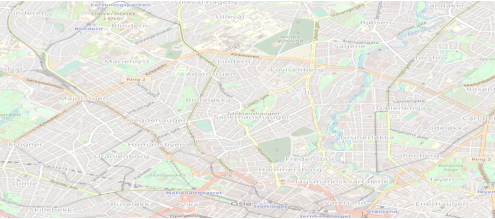
\includegraphics[width=\textwidth]{Images/empty_map.png}
         \caption{Start with a map without any locations or zones. This defines the bound from where to sample e-scooters.}
         \label{fig:instance_example:empty}
     \end{subfigure}
     \hfill
     \begin{subfigure}{0.49\textwidth}
         \centering
         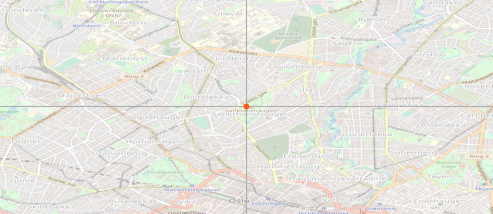
\includegraphics[width=\textwidth]{Images/map_only_zones.png}
         \caption{Each axis is split into sections of equal size to create the zones. The depot node is set to the center of the map (orange dot).}
         \label{fig:instance_example:only_zones}
     \end{subfigure}
     \hfill
     \begin{subfigure}{0.49\textwidth}
         \centering
         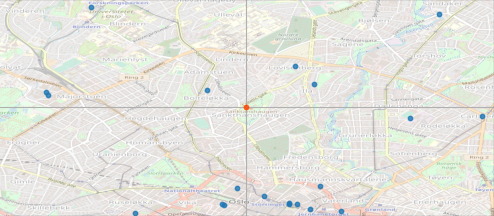
\includegraphics[width=\textwidth]{Images/map_scooters.png}
         \caption{A random sample of size equal to the number of e-scooters (blue dots) in the instance is taken from all e-scooters in \Cref{fig:all_data}.}
         \label{fig:instance_example:scoooters}
     \end{subfigure}
     \hfill
     \begin{subfigure}{0.49\textwidth}
         \centering
         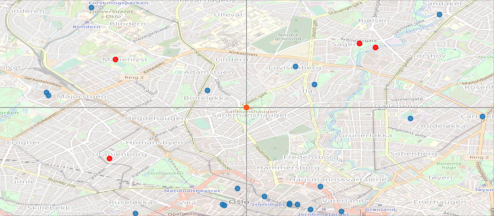
\includegraphics[width=\textwidth]{Images/map_locations.png}
         \caption{Created delivery locations (red dots) in the center of the zone with some random offset. The offset is set for illustrative purposes.}
         \label{fig:instance_example:loc}
     \end{subfigure}

    \caption{Steps to generate a test instance}
    \label{fig:instance_example}
\end{figure}
\break

For each zone, a deviation from the ideal state is computed to find the number of delivery nodes to be added. The ideal state of a zone is set to the $\textit{Number of E-scooters per Zone}$ parameter. This ensures an achievable total ideal state for the instance. In this report, demand patterns depending on geography and demography have not been analyzed. Consequently, the ideal state is the same for every zone in a given test instance. From the example in \Cref{fig:instance_example:scoooters} the zone in the upper right corner has an ideal state of five and currently has three e-scooters. Hence, two new delivery nodes are created as seen in \Cref{fig:instance_example:loc}. The position of the delivery nodes is set to the center of a zone with a small random deviation for visual purposes. The allocation of delivery nodes is independent of the battery capacity of the e-scooters already present in a zone. This is due to the fact that the number of e-scooters in a zone after every possible battery swap or rebalancing move is performed, should be equal to the ideal state for that zone. 

\subsection{Capacities and Shift Duration}
As the objective function does not include any minimization of time, either the shift duration or vehicle capacities must be binding constraints to limit the possible solutions of the model within the geographical area of the test instance. Further, to investigate the complexity of the problem with respect to how many nodes are visited, an appropriate value for the time constraint is necessary. For the test instances discussed in this report, the shift durations are significantly shorter than a regular workday, and are determined to reflect the proportion of e-scooters the service vehicles are able to handle during a shift. As the problem of finding a shift duration that corresponds to a solution visiting e.g. half of the nodes is almost as complex as the original problem, an approximation is used. A TSP optimization model using branch and bound with a short timeout is used for this problem. The solution to this model returns the shortest possible shift duration possible of visiting all locations. This result is used as an upper bound on the shift duration. To create instances visiting half of the locations, the shift is set to half of the amount of the TSP solution, as shown in Equation \eqref{eq:shiftDuration}. 
\begin{equation}
    \textit{Shift Duration} = \textit{upper bound on shift duration } * \% \textit{ of nodes to be visited }\label{eq:shiftDuration}
\end{equation}
\begin{equation}
    \begin{gathered}
        \textit{Battery Capacity} = \frac{\textit{Number of Locations with e-scooters}}{\textit{Number of Service Vehicles}}\\
        \textit{E-scooter Capacity} = \textit{max number of delivery locations in a zone}
    \end{gathered}\label{eq:capacities}
\end{equation}

The default value of the capacity for batteries is set to avoid it being a binding constraint. To ensure this, the capacity is set to the number of locations containing e-scooters divided by the number of service vehicles, as shown in Equation \eqref{eq:capacities}. The vehicles will then have the ability to visit all locations excluding the consideration of the time constraint. Similarly, the number of e-scooters a service vehicles can carry is capacitated by the maximum amount of delivery locations in a zone. 



\section{Example Solution to Test Instance}\label{example_solution}

This section aims to discuss the solution of the standard model on a selected test instance. The selected test instance contains 12 e-scooters placed in downtown Oslo. These e-scooters are distributed across four different zones. For the simplicity, the zones have the same ideal state of three per zone. The initial state of the test instance can be seen in \Cref{fig:example_instance}. 
\\
\begin{figure}[h]
    \centering
    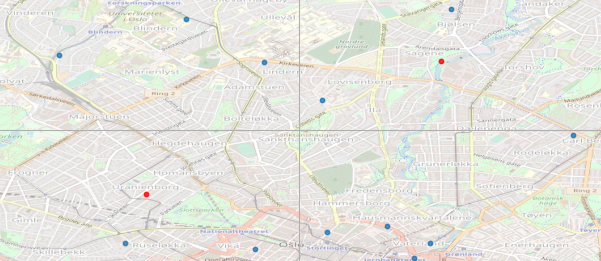
\includegraphics[width=15cm]{Images/example_instance.png}
    \caption{Initial state of the test instance}
    \label{fig:example_instance}
\end{figure}
\break

A selection of the input used in the example solution is summarized in \Cref{tab:param_example_solution}. $T_{max}$ is set to a value that makes it impossible for a single service vehicles to visit all locations. This makes the model prioritize the locations that yield the highest reward. The battery capacity of the service vehicles has been set to 6, adding up to the total number of e-scooters for all vehicles combined. Additionally, the total e-scooter capacity sums up to the number of possible rebalancing moves. 
\\
\begingroup
    \setlength{\tabcolsep}{10pt} % Default value: 6pt
    \renewcommand{\arraystretch}{1.9} % Default value: 1
    \begin{table}[h]
        \centering
        \caption{Parameters used in solution of test instance}
        \begin{tabular}{c|c|c}
            
             \textbf{Input} & \textbf{Symbol} & \textbf{Value}   \\
             \hline
             Number of e-scooters & $|\mathcal{L}|$ & 12\\
             \hline
             Number of service vehicles & $|\mathcal{V}|$ & 2\\
             \hline
             Shift duration & $T_{max}$ & 23\\
             \hline
             Battery capacity & $Q^B$ & 6\\
             \hline
             E-scooter capacity & $Q^S$ & 1\\
             
        \end{tabular}
        \label{tab:param_example_solution}
    \end{table}
\endgroup

The optimal solution for this test instance is visualized in \Cref{fig:example_solution}. The service vehicles swap the battery in some of the locations, and rebalance e-scooters in others. As intended, the solution is constrained by the duration of the shift. Both service vehicles follow similar paths. They visit five locations each, swapping batteries in three of them, and performing one rebalancing move. In nodes 3, 7 and 9 the battery of the e-scooters is swapped by vehicle 1. Furthermore, the e-scooter in node  5 is picked up in zone 4 where there is an excess of e-scooters and delivered to zone 2 where there is shortage. Consequently, vehicle 1 contributes to increasing the overall availability of e-scooters both by battery swaps and by moving an available e-scooter to a zone where the supply is needed.
\\
\begin{figure}[H]
    \hspace*{-1.7cm}
    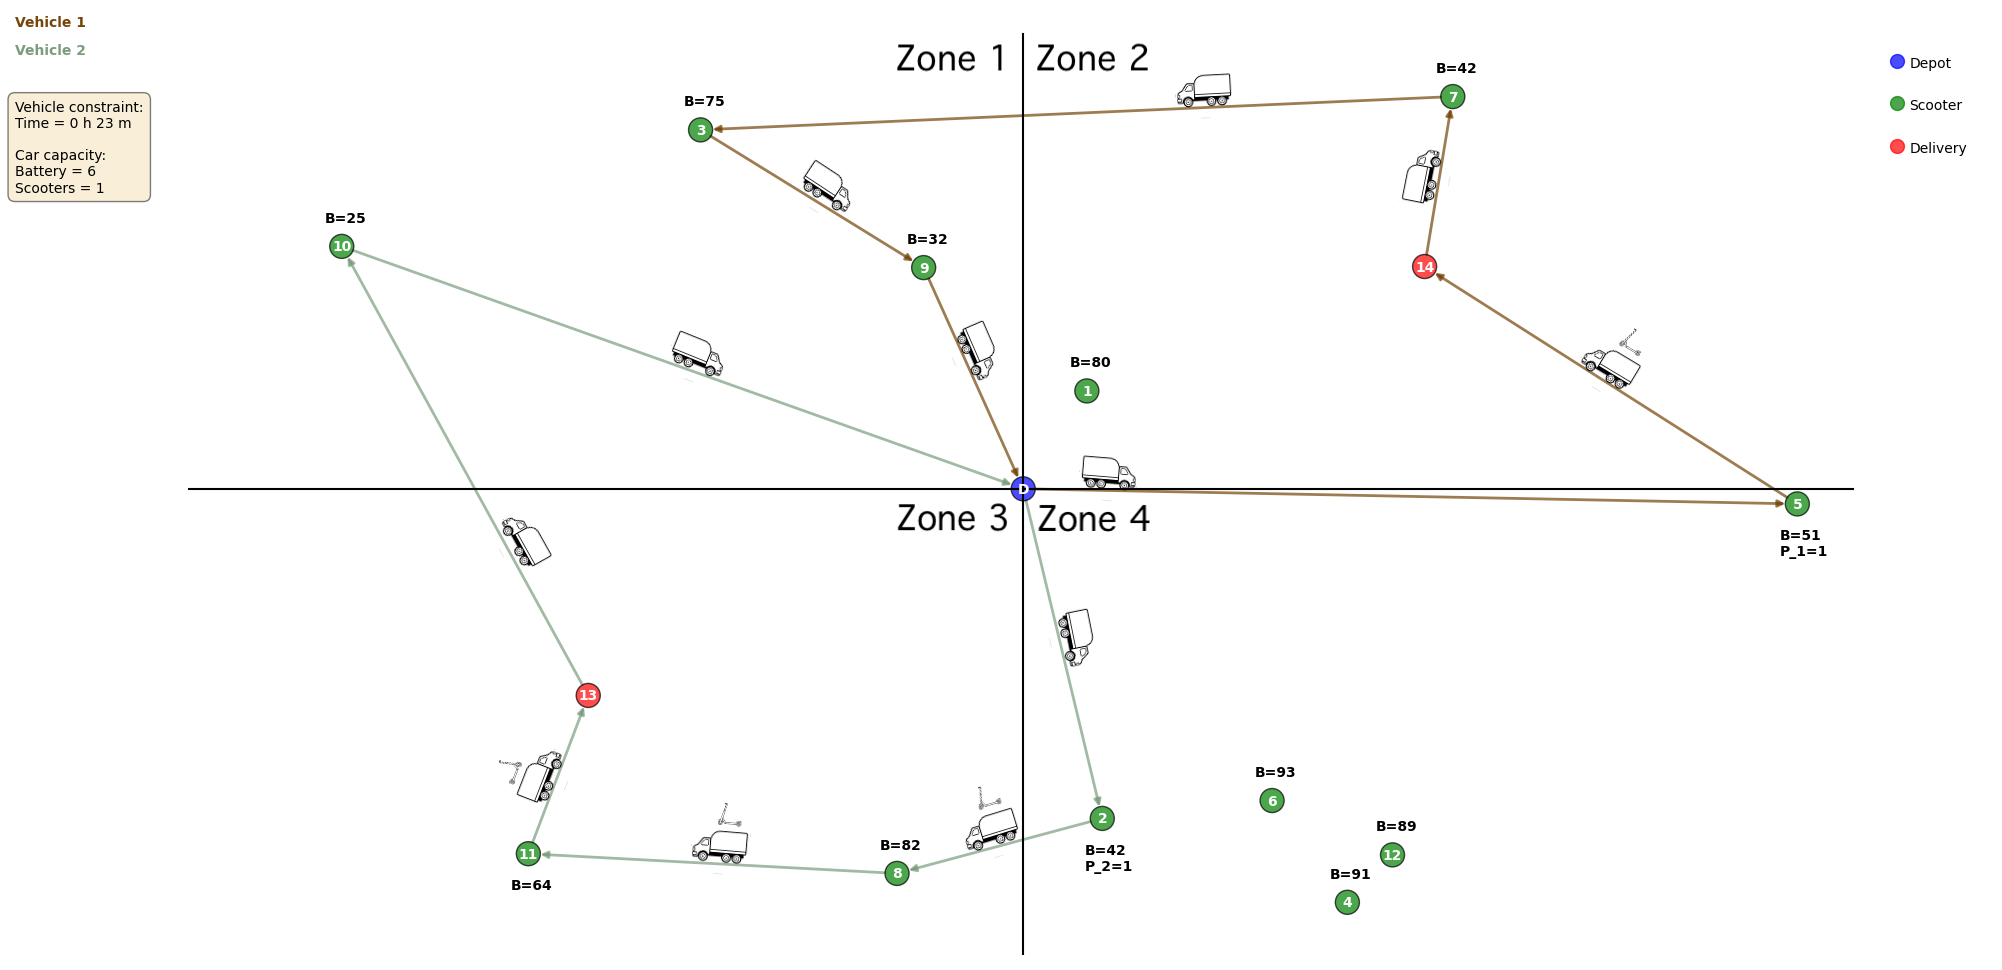
\includegraphics[width=18cm]{Images/example_solution.png}
    \caption{Solution to test instance}
    \label{fig:example_solution}
\end{figure}

The proposed solution leaves the four zones closer to their ideal state in the form of battery percentage. A summary of the deviation from the ideal state is presented in \Cref{tab:deviation_ex_sol}. An e-scooter with 100\% battery counts as 1 available e-scooter, while an e-scooter with 30\% capacity counts as 0.3. The difference between the total value of available e-scooters before and after the service vehicles have performed their routes is the total battery capacity added by the solution. The italic value denotes the excess of available e-scooters in the given zone, but is nevertheless counted as a contribution to the total deviation from the ideal state.
\\
\begingroup
    \setlength{\tabcolsep}{10pt} % Default value: 6pt
    \renewcommand{\arraystretch}{1} % Default value: 1
    \begin{table}[H]
        \centering
        \caption{Deviation from ideal state before and after the solution}
        \begin{tabular}{c|c|c}
            
             \textbf{Zone} & \textbf{Deviation Before} & \textbf{Deviation After}   \\
             \hline
             1 & 1.68 & 0\\
             2 & 1.78 & 0.20\\
             3 & 1.54 & 0\\
             4 & \textit{0.66} & 0.27\\
             \hline
             Total & 5.66 & 0.47\\
             \thickhline
        \end{tabular}
        \label{tab:deviation_ex_sol}
    \end{table}
\endgroup

From the results in \cref{tab:deviation_ex_sol}, the conclusion is that the proposed solution to the test instance significantly improves the availability of e-scooters. While the total deviation from the ideal states was 5.66 prior to the planning, it is reduced to 0.47 afterwards. The difference between these two values, 5.19, can be viewed as the total amount of added availability of e-scooters that the solution contributes with. Referring to the previous paragraph, 5.19 e-scooters equal 519\% of battery capacity available. 

This example solution was run on a relatively small test instance for the purpose of visualization. However, the behavior of the solution varies greatly for different sizes of test instances and parameters. A further analysis of the variety of solutions is presented in Chapter \ref{comp_study}.
